\documentclass[../../main.tex]{subfiles}

\begin{document}

\section{Motivation}

Machine learning models have demonstrated immense success in a variety of applications, generating data-driven  predictions in domains such as computer vision, robotics, weather forecasting. While the success of these models is undeniable, they often to lack the ability to quantify the uncertainty in the predictions. This is a major drawback in the deployment of these models in real-world applications, for instance, in weather forecasting,  the uncertainty of the prediction of the weather is arguably as valuable as the prediction itself. Or in the case of robotics where estimating the uncertainty of objects in the environment is crucial for safe navigation and decision-making.

In this work, we develop and test models that are not only capable of making accurate predictions but also \textbf{aware of the uncertainty associated with their prediction}.

Furthermore, we would like the model to possess properties that enhance its ability to learn and generalize on data with strong patterns or periodicity, such as spatio-temporal data. Accurately capturing these patterns is crucial for modelling many real world tasks such as:

\begin{itemize}
	\item \textbf{Climate modelling}: parameters such as temperature, humidity, and pressure have strong spatio-temporal dependencies which exhibit periodic patterns. Accurately modelling these patterns is crucial for predicting weather patterns.
	\item \textbf{Time series forecasting}: Many real world time series data exhibit periodic patterns, such as stock prices, energy consumption, and traffic data which have daily, weekly, and yearly periodicity. 
	\item \textbf{Image processing}: Images have strong spatial dependencies, such as textures, edges and blobs which play a large role in characterizing the underlying structure of the data.
\end{itemize}


To achieve this, we insert some desirable inductive biases that help the model to generalize better and be more interpretable. These properties are:

\textbf{Flexible}: \emph{The model should be able to work on a variety of data types}. As long as a data point can be represented as a vector, the model should be able to operate on it. This allows the model to be used in a variety of applications and domains.

\textbf{Scalable}: \emph{The model should be able to learn large datasets and scale to as many inputs}. Which is not the case with many traditional models such as Large Language Models (LLMs) which are usually limited to a max number of tokens. Another aspect of scalability is the ability learn high-dimensional data with good computational efficiency.


\textbf{Permutation Invariant}: \emph{The prediction of the model should not change if the order of the input data is changed}. When each data point contains the information about input and output pairs, the model should not care about the order in which they are fed into the model. For example, in the case of a weather forecasting model, which uses data from multiple weather stations, the model should not care about the order in which the data from the weather stations is fed into the model, thus making the model permutation invariant.

\textbf{Translation Equivariant}: \emph{Shifting the input data by a constant amount should result in a constant shift in the predictions}. 

\begin{figure}[H]
	\centering
	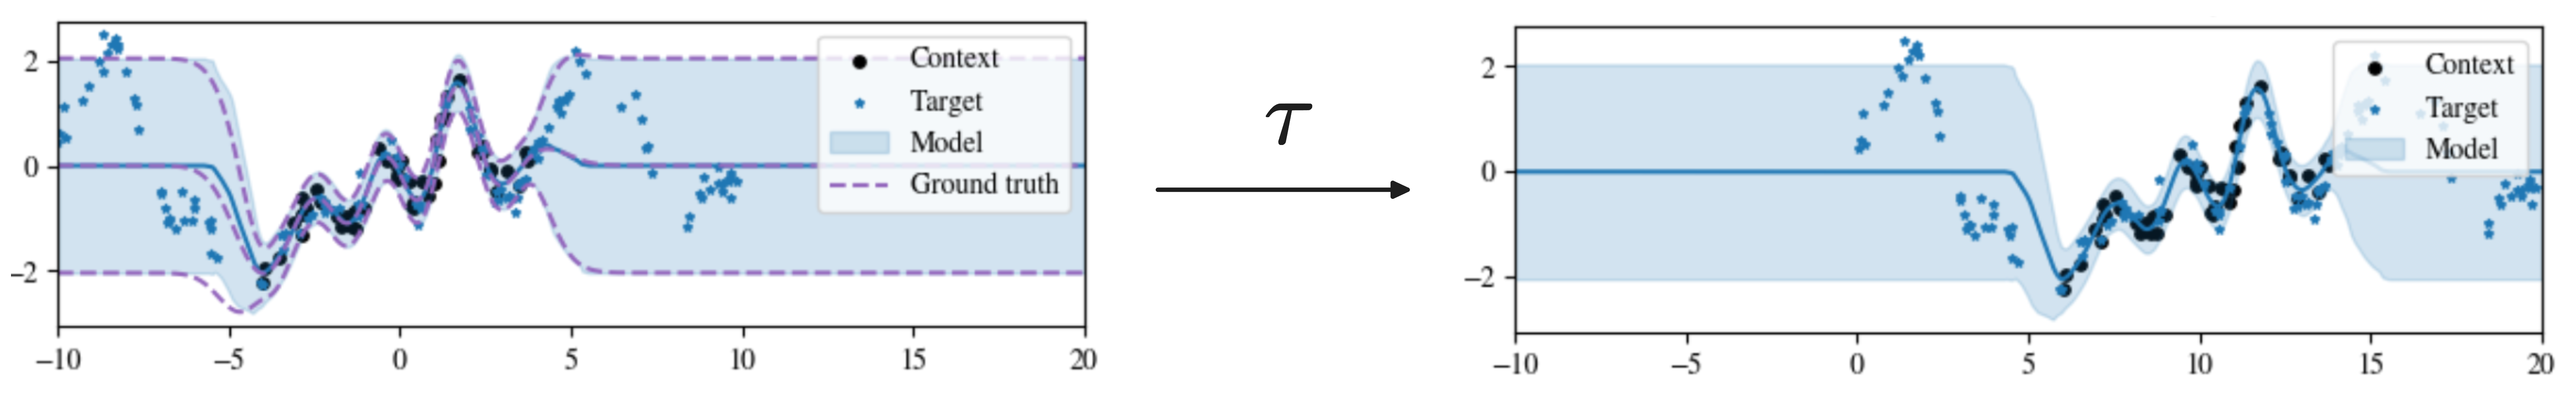
\includegraphics[width=0.9\textwidth]{./te.png}
	\caption{The Translation Equivariant property on a 1D dataset.}
	\label{fig:te}
\end{figure}


\autoref{fig:te} illustrates this property, when the input data on the left plot is shifted by a constant amount, the prediction should also shift by the same amount (right). Mathematical, a model $f$ is translation equivariant if it satisfies the following property:

\begin{align}
	&f: \bm{x} \rightarrow (\bm{x}, \bm{\hat{y}}) \\
	&f: \bm{x} + \bm{\tau} \rightarrow (\bm{x} + \bm{\tau}, \bm{\hat{y}})
\end{align}

where $\bm{x}$ is the input and $\bm{\hat{y}}$ is the output and $\bm{\tau}$ is a constant shift in the input. Such property allows the model to be more robust and generalize better to unseen data, particularly in the case of stationary data.


\textbf{Off the Grid Generalization}: \emph{The model should be capable of operating on off-the-grid data points}. Off the grid data points are the data points that are not in a regular gridded structure, such as images that have missing pixel values. Traditional models like Convolutional Neural Networks (CNNs) are not able to operate on off-the-grid data points since they require a regular structure to apply the convolution operation. By making the model off-the-grid generalizable, we can create models that can work on many types of datasets and easily handle missing data points. Furthermore, aiding in the performance of the model outside the context data. Applications such as image inpainting can particularly benefit from off-the-grid generalization.


\section{Aims and Objectives}

Neural Processes (NPs) \parencite{garnelo2018neural} are a class of uncertainty aware models that can be used for meta-learning. The framework undermining NPs is general purpose, whilst fulfilling the properties discussed earlier. Due to their flexibility, the NP architectures can be easily adapted to incorporate various backbone models and inductive biases. 

In this work, we aim to implement and compare two different neural network architectures for Neural Processes, the first being based on a Convolutional Neural Network (CNN) called Convolutional Neural Processes (ConvNP) and the second being based on a Transformer architecture called Transformer Neural Processes (TNP). Our objective is to compare the performance of two models on a variety of datasets, focusing on their generalization capabilities and scalability.

We introduce extra inductive biases into the TNP to enhance its ability to generalize. Furthermore, we explore new Transformer architectures that have better computational efficiency compared to the original Transformer architecture.

Our objective is to develop a comprehensive understanding of the properties of these models. We aim to identify  the best practices for using these models in different scenarios, highlighting contexts where they perform well and where they do not. This investigation will provide us valuable insights into the capabilities of these models and how they can be deployed in real-world applications.





\ifSubfilesClassLoaded{%
    \printbibliography{}
}{} 


\end{document}